%-------------------------------------------------------------------------------
%                                PREAMBLE
%-------------------------------------------------------------------------------
\documentclass[usenames,dvipsnames,svgnames,10pt,aspectratio=169]{beamer}
%
\usefonttheme{professionalfonts}
% This theme uses TIKZ: compile twice with PDFLaTeX or LuaLaTeX.
%
%  Options:
%  - [clean]:    clean slides, i.e. logos and footbar are removed
%  - [kth]:      footbar style inspierd to the official KTH template
%  - [nicewave]: a different style of wave is used (not approved by FLOW)
%
\usetheme[clean]{flow}

\usepackage{tikz}
\usepackage{pgfplots}
\usepgfplotslibrary{polar}

\usepackage{hyperref,graphicx,lmodern}
\usepackage[utf8]{inputenc}
\usepackage{media9}
\usepackage{xcolor}
\usepackage{stmaryrd}
\usepackage{nicefrac}
\usepackage{multimedia}
\usepackage{multicol}
\usepackage{upgreek}
\usepackage[]{bm}
\usepackage[]{url}
\usepackage[]{animate}
\usepackage{amsmath}

\graphicspath{{imgs/}}
\setbeamertemplate{blocks}[rounded][shadow=true]


\usepackage[]{listings}

\definecolor{codegreen}{rgb}{0,0.6,0}
\definecolor{codegray}{rgb}{0.5,0.5,0.5}
\definecolor{codepurple}{rgb}{0.58,0,0.82}
\definecolor{backcolour}{rgb}{1.0, 1.0, 1.0}

\lstdefinestyle{mystyle}{
  backgroundcolor=\color{backcolour},
  commentstyle=\color{codegreen},
  keywordstyle=\color{magenta},
  numberstyle=\tiny\color{codegray},
  stringstyle=\color{codepurple},
  basicstyle=\ttfamily\footnotesize,
  breakatwhitespace=false,
  breaklines=true,
  captionpos=b,
  keepspaces=true,
  numbers=left,
  numbersep=5pt,
  showspaces=false,
  showstringspaces=false,
  showtabs=false,
  tabsize=2
}

\lstset{style=mystyle}


%-------------------------------------------------------------------------------
%                                TITLE PAGE
%-------------------------------------------------------------------------------
\title[Nonlinear physics] % Short title used in footline
{
	Introduction au calcul scientifique
}

\author[J.-Ch.~Loiseau] % Presenting author in short form used in footline
{
	\underline{Jean-Christophe Loiseau}
}
% - Give the names in the same order as the appear in the paper.
% - Underline the presenting author.

\institute[unused]
{
	\url{jean-christophe.loiseau@ensam.eu} \\
	Laboratoire DynFluid \\
	Arts et M\'etiers, France.
}
% Keep it simple, no one is interested in your street address.

% University logo(s)
\logot{\includegraphics[width=.128\paperwidth]{DynFluid_logo}}  % Top logo
\logob{\includegraphics[width=0.128\paperwidth]{ENSAM_logo}} % Bottom logo
% \logoc[{\includegraphics[width=.128\paperwidth]{limsi}}]{\includegraphics[width=.128\paperwidth]{limsi}} % Corner logo
%
% Cover image: \cvrimg{x position}{y position}{cover image}
\cvrimg{.77}{.8}{\includegraphics[width=.4\paperwidth]{cover.png}}

\date[unused]{Physique non-lin\'eaire -- 2019-2020}

\begin{document}

\titleframe	% Print the title as the first slide

%-------------------------------------------------------------------------------
%                           PRESENTATION SLIDES
%-------------------------------------------------------------------------------

\begin{frame}[t, c]{Recherche de racines}{}
	\begin{minipage}{.68\textwidth}
    De nombreux problèmes d'ingénierie nécessitent de trouver les valeurs de $x$ telles que
    %
    \[
    f(x) = 0
    \]
    %
    avec $x \in \mathbb{R}$ et $f : \mathbb{R} \to \mathbb{R}$.
    Les valeurs de $x$ satisfaisant cette équations ont appelées les \alert{\textbf{racines de la fonction $f$}}.
	\end{minipage}%
	\hfill
	\begin{minipage}{.28\textwidth}
    \centering
    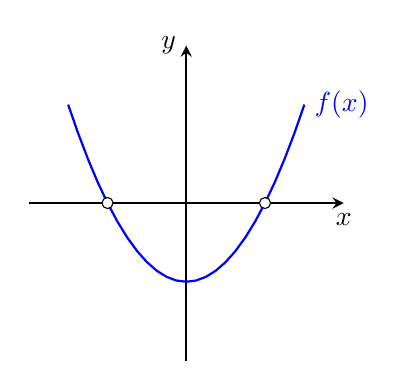
\begin{tikzpicture}[>=stealth]
      \draw[->, thick] (-2, 0) -- (2, 0) node[below] {$x$};
      \draw[->, thick] (0, -2) -- (0, 2) node[left] {$y$};

      \draw[-, blue, thick, variable=\x, domain=-1.5:1.5] plot (\x, {(\x-1)*(\x+1)}) node[right] {$f(x)$};

      \node[circle, fill=white, draw=black, inner sep=0pt, minimum size=4pt] (a) at (1, 0) {};
      \node[circle, fill=white, draw=black, inner sep=0pt, minimum size=4pt] (a) at (-1, 0) {};
    \end{tikzpicture}
	\end{minipage}

	\vspace{1cm}
\end{frame}

\begin{frame}[t, c]{Recherche de racines}{Quelques exemples}
  \begin{minipage}{.68\textwidth}
    Les pertes de charge dans une conduite peuvent être modélisées par
    %
    \[
    \Delta p = f_D \dfrac{\rho V^2}{2} \dfrac{L}{D}
    \]
    %
    où $f_D$ est la coefficient de friction de Darcy-Weisbach permettant de prendre en compte la rugosité des parois des la conduite.
  \end{minipage}%
  \hfill
  \begin{minipage}{.28\textwidth}
  \end{minipage}
\end{frame}

\begin{frame}[t, c]{Recherche de racines}{Quelques exemples}
  \begin{minipage}{.68\textwidth}
    Pour une taille caractéristique $\epsilon$ des rugosités, ce coefficent est solution de l'équation empirique de Colebrook
    %
    \[
    \dfrac{1}{\sqrt{f_D}} = 2 \log_{10} \left( \dfrac{\epsilon}{3.7D} + \dfrac{2.51}{Re \sqrt{f_D}} \right).
    \]
    %
    Cette équation n'admet pas de solution analytique.
    Ses racines doivent alors être calculées numériquement.

  \end{minipage}%
  \hfill
  \begin{minipage}{.28\textwidth}
    \centering
    \includegraphics[width=\textwidth]{Moody_chart}
  \end{minipage}

  \vspace{1cm}
\end{frame}

\begin{frame}[t, c]{Recherche de racines}{Quelques exemples}
  \begin{minipage}{.68\textwidth}
    Une possible équation d'état pour un gaz non-idéal est donnée par celle de van der Walls
    %
    \[
    p - \dfrac{RT}{V-b} + \dfrac{a}{V^2} = 0
    \]
    %
    En deça d'une température critique, un équilibre liquide-vapeur peut exister.
    Le volume molaire $V$ de chaque phase est alors déterminé en calculant les racines de l'équation ci-dessus.
  \end{minipage}%
  \hfill
  \begin{minipage}{.28\textwidth}
    \centering
  \end{minipage}

  \vspace{1cm}
\end{frame}

%%%%%
%%%%%
%%%%%
%%%%%
%%%%%

\begin{frame}[t, c]{Recherche de racines}{Fonctions polynômiales}
  \begin{minipage}{.68\textwidth}
    Soit $f : \mathbb{R} \to \mathbb{R}$ une fonction quadratique
    %
    \[
    f(x) = x^2 + ax + b
    \]
    %
    avec $a$ et $b$ des constantes (réelles ou complexes).
    Ses racines sont données par
    %
    \[
    x = \dfrac{-a \pm \sqrt{\Delta}}{2}
    \]
    %
    avec $\Delta = a^2 - 4b$ le discriminant.
  \end{minipage}%
  \hfill
  \begin{minipage}{.28\textwidth}
    \centering
    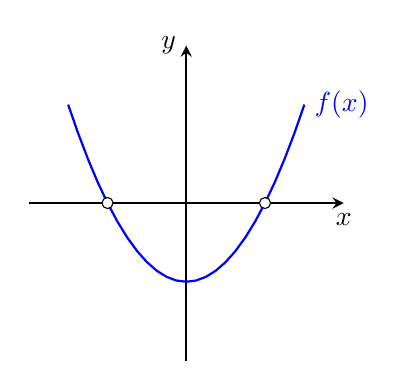
\begin{tikzpicture}[>=stealth]
      \draw[->, thick] (-2, 0) -- (2, 0) node[below] {$x$};
      \draw[->, thick] (0, -2) -- (0, 2) node[left] {$y$};

      \draw[-, blue, thick, variable=\x, domain=-1.5:1.5] plot (\x, {(\x-1)*(\x+1)}) node[right] {$f(x)$};

      \node[circle, fill=white, draw=black, inner sep=0pt, minimum size=4pt] (a) at (1, 0) {};
      \node[circle, fill=white, draw=black, inner sep=0pt, minimum size=4pt] (a) at (-1, 0) {};
    \end{tikzpicture}
  \end{minipage}

  \vspace{1cm}
\end{frame}

\begin{frame}[t, c]{Recherche de racines}{Fonctions polynômiales}
  \begin{minipage}{.68\textwidth}
    On peut montrer que les racines de $f$ sont les valeurs propres de la matrice compagnon
    %
    \[
    \bm{C}
    =
    \begin{bmatrix}
      0 & -b \\
      1 & -a
    \end{bmatrix}.
    \]
    %
    Cette équivalence existe pour n'importe quelle fonction polynômiale à une variable.
  \end{minipage}%
  \hfill
  \begin{minipage}{.28\textwidth}
    \centering
    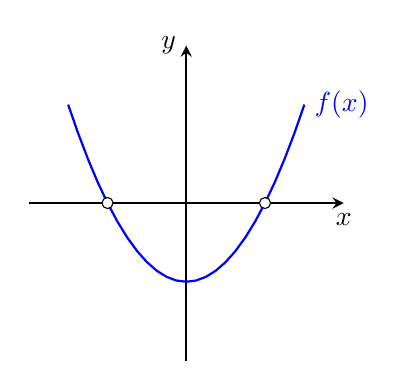
\begin{tikzpicture}[>=stealth]
      \draw[->, thick] (-2, 0) -- (2, 0) node[below] {$x$};
      \draw[->, thick] (0, -2) -- (0, 2) node[left] {$y$};

      \draw[-, blue, thick, variable=\x, domain=-1.5:1.5] plot (\x, {(\x-1)*(\x+1)}) node[right] {$f(x)$};

      \node[circle, fill=white, draw=black, inner sep=0pt, minimum size=4pt] (a) at (1, 0) {};
      \node[circle, fill=white, draw=black, inner sep=0pt, minimum size=4pt] (a) at (-1, 0) {};
    \end{tikzpicture}
  \end{minipage}

  \vspace{1cm}
\end{frame}


\begin{frame}[t, c]{Recherche de racines}{Fonctions polynômiales}
  \begin{minipage}{.68\textwidth}
    Soit $f : \mathbb{R} \to \mathbb{R}$ une fonction polynomiale donnée par
    %
    \[
    f(x) = x^n + c_{n-1} x^{n-1} + c_{n-2} x^{n-2} + \cdots + c_1 x + c_0.
    \]
    %
    Ses racines sont les valeurs propres de la matrice
    %
    \[
    \bm{C}
    =
    \begin{bmatrix}
      0 & 0 & \cdots & 0 & -c_0 \\
      1 & 0 & \cdots & 0 & -c_1 \\
      0 & 1 & \cdots & 0 & -c_2 \\
      \vdots & \vdots & \ddots & \vdots & \vdots \\
      0 & 0 & \cdots & 1 & -c_{n-1}
    \end{bmatrix}.
    \]
    %
    Il est important de noter que l'on suppose $c_n = 1$.
  \end{minipage}%
  \hfill
  \begin{minipage}{.28\textwidth}
    \centering
    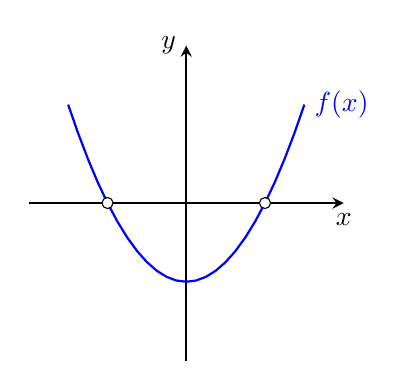
\begin{tikzpicture}[>=stealth]
      \draw[->, thick] (-2, 0) -- (2, 0) node[below] {$x$};
      \draw[->, thick] (0, -2) -- (0, 2) node[left] {$y$};

      \draw[-, blue, thick, variable=\x, domain=-1.5:1.5] plot (\x, {(\x-1)*(\x+1)}) node[right] {$f(x)$};

      \node[circle, fill=white, draw=black, inner sep=0pt, minimum size=4pt] (a) at (1, 0) {};
      \node[circle, fill=white, draw=black, inner sep=0pt, minimum size=4pt] (a) at (-1, 0) {};
    \end{tikzpicture}
  \end{minipage}

  \vspace{1cm}
\end{frame}


\begin{frame}[t, c, fragile]{Recherche de racines}{Fonctions polynômiales}
  \begin{minipage}{.68\textwidth}
    \begin{lstlisting}[language=Python]
      from numpy.polynomial import Polynomial

      # --> Coefficients du polynome f(x) = x**2 - 1.
      coefs = [-1, 0, 1]

      # --> Creation du polynome.
      p = Polynomial(coefs)

      # --> Calcul des racines.
      roots = p.roots()
    \end{lstlisting}
  \end{minipage}%
  \hfill
  \begin{minipage}{.28\textwidth}
    \centering
    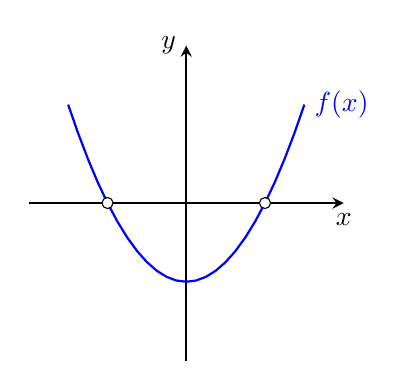
\begin{tikzpicture}[>=stealth]
      \draw[->, thick] (-2, 0) -- (2, 0) node[below] {$x$};
      \draw[->, thick] (0, -2) -- (0, 2) node[left] {$y$};

      \draw[-, blue, thick, variable=\x, domain=-1.5:1.5] plot (\x, {(\x-1)*(\x+1)}) node[right] {$f(x)$};

      \node[circle, fill=white, draw=black, inner sep=0pt, minimum size=4pt] (a) at (1, 0) {};
      \node[circle, fill=white, draw=black, inner sep=0pt, minimum size=4pt] (a) at (-1, 0) {};
    \end{tikzpicture}
  \end{minipage}

  \vspace{1cm}
\end{frame}

\begin{frame}[t, c]{Recherche de racines}{Fonctions non-polynômiales}
  \begin{minipage}{.68\textwidth}
    Pour une fonction $f : \mathbb{R} \to \mathbb{R}$ non-polynômiale, il est rare que les racines puissent être écrites de façon analytique.
    Il est alors nécessaire de recourir à des méthodes numériques pour les approximer.

    \bigskip

    \textbf{Exemple :} Trouvez les racines de la fonction
    %
    \[
    f(x) = a - x + b \sin(x)
    \]
    %
    avec $a$ et $b$ des constantes données par le problème.
  \end{minipage}%
  \hfill
  \begin{minipage}{.28\textwidth}
    \centering
    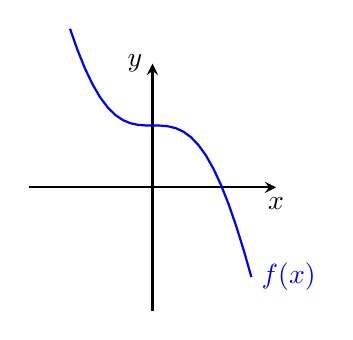
\begin{tikzpicture}[>=stealth]
      \draw[->, thick] (-pi/2, 0) -- (pi/2, 0) node[below] {$x$};
      \draw[->, thick] (0, -pi/2) -- (0, pi/2) node[left] {$y$};

      \draw[-, blue, variable=\x, domain=-pi/3:4*pi/10, thick] plot (\x, {pi/4 - 2*\x + sin(2*\x r)}) node[right] {$f(x)$};
    \end{tikzpicture}
  \end{minipage}

\end{frame}

\begin{frame}[t, c]{Recherche de racines}{Graphe de la fonction}
  \begin{minipage}{.68\textwidth}
    Pour une fonction $f : \mathbb{R} \to \mathbb{R}$, l'approche la plus simple pour voir si il existe des racines dans l'intervalle $\left[a, b\right]$ consiste à tracer le graphe de la fonction $f(x)$.

    \bigskip

    Cette méthode ne permet pas techniquement de calculer les racines mais uniquement de visualiser si il en existe.
    Elle nous permet donc d'estimer \emph{a priori} combien de racines il y'a et quelles sont leurs valeurs.
  \end{minipage}%
  \hfill
  \begin{minipage}{.28\textwidth}
    \centering
    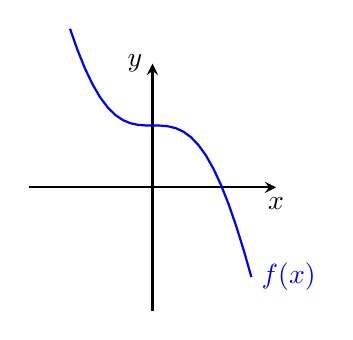
\begin{tikzpicture}[>=stealth]
      \draw[->, thick] (-pi/2, 0) -- (pi/2, 0) node[below] {$x$};
      \draw[->, thick] (0, -pi/2) -- (0, pi/2) node[left] {$y$};

      \draw[-, blue, variable=\x, domain=-pi/3:4*pi/10, thick] plot (\x, {pi/4 - 2*\x + sin(2*\x r)}) node[right] {$f(x)$};
    \end{tikzpicture}
  \end{minipage}

  \vspace{1cm}
\end{frame}


\begin{frame}[t, c, fragile]{Recherche de racines}{Graphe de la fonction}
  \begin{minipage}{.68\textwidth}
    \begin{lstlisting}[language=Python]
      import numpy as np
      import matplotlib.pyplot as plt

      # --> Definition de la fonction
      f = lambda x: np.pi/4 - x + np.sin(x)

      # --> Definition de l'intervalle
      a, b = -np.pi, np.pi
      x = np.linspace(a, b, 1024)

      # --> Trace le graphe de la fonction.
      plt.plot(x, f(x))
      plt.axhline(0, c='black') # Ligne y=0.
      plt.show()
    \end{lstlisting}
  \end{minipage}%
  \hfill
  \begin{minipage}{.28\textwidth}
    \centering
    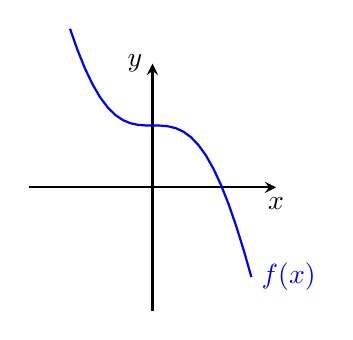
\begin{tikzpicture}[>=stealth]
      \draw[->, thick] (-pi/2, 0) -- (pi/2, 0) node[below] {$x$};
      \draw[->, thick] (0, -pi/2) -- (0, pi/2) node[left] {$y$};

      \draw[-, blue, variable=\x, domain=-pi/3:4*pi/10, thick] plot (\x, {pi/4 - 2*\x + sin(2*\x r)}) node[right] {$f(x)$};
    \end{tikzpicture}

  \end{minipage}
\end{frame}

\begin{frame}[t, c]{Recherche de racines}{Méthodes numériques}
  \begin{minipage}{.68\textwidth}
    Il existe de nombreux algorithmes pour calculer les racines d'une fonction $f : \mathbb{R} \to \mathbb{R}$.
    Chacun d'eux repose sur différentes hypothèses concernant $f$ (e.g. continuité, dérivabilité, etc) conduisant à plus ou moins d'efficacité et/ou de robustesse.
  \end{minipage}%
  \hfill
  \begin{minipage}{.28\textwidth}
  \end{minipage}

  \vspace{1cm}
\end{frame}


\begin{frame}[t, c, fragile]{Recherche de racines}{Méthodes numériques}
  \begin{minipage}{.68\textwidth}
    Dans la suite, nous discuterons des trois méthodes les plus populaires, à savoir :
    \begin{itemize}
    \item la méthode de la bissection (ou dichotomie),
    \item la méthode de Newton-Raphson,
    \item la méthode de la sécante.
    \end{itemize}

    \bigskip

    Elles sont toutes disponibles dans \verb+scipy.optimize+ via l'interface unifiée \verb+root_scalar+.
  \end{minipage}%
  \hfill
  \begin{minipage}{.28\textwidth}
    \centering
    \includegraphics[width=\textwidth]{scipy_logo}
  \end{minipage}
\end{frame}

\begin{frame}[t, c]{Recherche de racines}{Méthode de la bissection}
  \begin{minipage}{.68\textwidth}
    \textbf{Théorème de Bolzano :} Pour toute fonction continue $f : \left[a, b \right] \to \mathbb{R}$ telle que $f(a)$ et $f(b)$ soient de signe opposé, il existe au moins un réel $c \in \left[a, b\right]$ tel que $f(c) = 0$.
  \end{minipage}%
  \hfill
  \begin{minipage}{.28\textwidth}
  \end{minipage}
\end{frame}

\begin{frame}[t, c, fragile]{Recherche de racines}{Méthode de la bissection}
  \begin{minipage}{.68\textwidth}
    Supposons que les conditions pour que le théorème de Bolzano soit applicable sont vérifiées.
    Il est alors possible d'approximer numériquement une racine de $f(x)$ à l'aide l'algorithme ci-dessous.

    \bigskip

    \begin{lstlisting}[language=Python]
      while abs(b-a) < tol:
          c = (a+b) / 2
          if (f(a) * f(b) < 0):
              b = c
          else:
              a = c
    \end{lstlisting}

    C'est ce que l'on appelle \textbf{\alert{méthode de la bissection}} ou \textbf{\alert{méthode de la dichotomie}}.
  \end{minipage}%
  \hfill
  \begin{minipage}{.28\textwidth}
  \end{minipage}
\end{frame}

\begin{frame}[t, c]{Recherche de racines}{Méthode de la bissection}
  \begin{minipage}{.68\textwidth}
    A chaque étape, l'erreur d'approximation de la racine est divisée par un facteur 2.
    Après $n$ itérations, on a donc
    %
    \[
    e_n = \dfrac{\vert b - a \vert}{2^{n+1}}.
    \]

    \bigskip

    La méthode de la bissection jouit d'une grande robustesse mais converge \textbf{\alert{linéairement}} et peut donc nécessiter beaucoup d'itérations avant d'arriver au résultat.
    
  \end{minipage}%
  \hfill
  \begin{minipage}{.28\textwidth}
  \end{minipage}
\end{frame}

\begin{frame}[t, c, fragile]{Recherche de racines}{Méthode de la bissection}
  \begin{lstlisting}[language=Python]
    import numpy as np
    from scipy.optimize import root_scalar

    # --> Definition de la fonction.
    f = lambda x : np.pi/4 - x + np.sin(x)

    # --> Recherche des racines.
    sol = root_scalar(f, bracket=[0, np.pi], method="bisect")

    # --> Extrait differentes informations.
    x = sol.root # Racine obtenue.
    niter = sol.iterations # Nombre d'iterations.
    nfev = sol.functions_calls # Nombre d'appels de f(x).
  \end{lstlisting}
\end{frame}

\begin{frame}[t, c]{Recherche de racines}{Méthode de Newton-Raphson}
  \begin{minipage}{.68\textwidth}
    La méthode de la bissection repose uniquement sur l'hypothèse de continuité et n'utilise comme information que le signe de $f(x)$ aux bornes des intervalles (d'où sa lente convergence).

    \bigskip

    Si l'on suppose que $f : \mathbb{R} \to \mathbb{R}$ est également dérivable, alors il est possible de designer un algorithme plus efficace : la \alert{\textbf{méthode de Newton-Raphson}}.
  \end{minipage}%
  \hfill
  \begin{minipage}{.28\textwidth}
  \end{minipage}

  \vspace{1cm}
\end{frame}

\begin{frame}[t, c]{Recherche de racines}{Méthode de Newton-Rapshon}
  \begin{minipage}{.68\textwidth}
    Supposons que l'on ait une bonne estimation $x_0$ de la racine que l'on cherche.
    Au voisinage de $x_0$, on peut alors écrire
    %
    \[
    f(x) \simeq f(x_0) + f^{\prime}(x_0) \left(x - x_0 \right).
    \]
    %
    Posons $g_0(x) = f(x_0) + f^{\prime}(x_0) \left( x - x_0 \right)$ et cherchons sa racine.
  \end{minipage}%
  \hfill
  \begin{minipage}{.28\textwidth}
  \end{minipage}

  \vspace{1cm}
\end{frame}

\begin{frame}[t, c]{Recherche de racines}{Méthode de Newton-Raphson}
  \begin{minipage}{.68\textwidth}
    Il est facile de montrer que la racine de $g_0(x)$ est donnée par
    %
    \[
    x_1 = x_0 - \dfrac{f(x_0)}{f^{\prime}(x_0)}.
    \]
    %
    Si $x_0$ est une bonne estimation de la racine de $f(x)$, alors $x_1$ tend à être encore meilleure.
    On peut ensuite répéter ce processus à l'infini et montrer que la convergence est quadratique.
  \end{minipage}%
  \hfill
  \begin{minipage}{.28\textwidth}
  \end{minipage}
\end{frame}

\begin{frame}[t, c]{Recherche de racines}{Méthode de Newton-Raphson}
  \centering
  \includegraphics[width=.8\textwidth]{Newton_method}
\end{frame}

\begin{frame}[t, c, fragile]{Recherche de racines}{Méthode de Newton-Raphson}
  \begin{minipage}{.68\textwidth}
    Si l'on écrit ce processus en pseudocode, on obtient alors l'algorithme ci-dessous.

    \bigskip

    \begin{lstlisting}[language=Python]
      while abs(f(x)) < tol:
           x = x - f(x) / fprime(x)
    \end{lstlisting}

    \bigskip

    En pratique, le code est légèrement plus compliqué puisque l'on doit vérifier que $f^{\prime}(x)$ n'est pas nulle.
    On peut également ajouter une limite au nombre d'itérations.
  \end{minipage}%
  \hfill
  \begin{minipage}{.28\textwidth}
  \end{minipage}
\end{frame}

\begin{frame}[t, c, fragile]{Recherche de racines}{Méthode de Newton-Raphson}
  \begin{lstlisting}[language=Python]
    import numpy as np
    from scipy.optimize import root_scalar
    
    # --> Definition de la fonction et de sa derivee.
    f = lambda x : np.pi/4 - x + np.sin(x)
    df = lambda x: -1 + np.cos(x)
    
    # --> Recherche des racines.
    sol = root_scalar(
        f,              # Fonction f(x).
        fprime=df,      # Derivee de la fonction.
        x0=np.pi/2,     # Point de depart.
        method="newton"
    )

  \end{lstlisting}
\end{frame}

\begin{frame}[t, c, fragile]{Recherche de racines}{Méthode de Newton-Raphson}
  \begin{minipage}{.68\textwidth}
    \begin{lstlisting}[language=Python]
      import numpy as np
      from scipy.optimize import root_scalar
      from scipy.optimize import approx_frpime
      
      # --> Definition de la fonction et de sa derivee.
      f = lambda x : np.pi/4 - x + np.sin(x)
      df = lambda x : approx_fprime(x, f, 1e-6)
      
      # --> Recherche des racines.
      sol = root_scalar(
          f,              # Fonction f(x).
          fprime=df,      # Derivee de la fonction.
          x0=np.pi/2,     # Point de depart.
          method="newton"
      )
    \end{lstlisting}
  \end{minipage}%
  \hfill
  \begin{minipage}{.28\textwidth}
  \end{minipage}
\end{frame}

\begin{frame}[t, c]{Recherche de racines}{Méthode de la sécante}
  \begin{minipage}{.68\textwidth}
    La méthode de Newton-Raphson est sans doute la méthode la plus efficace pour calculer des racines.
    Elle nécessite néanmoins la connaissance de $f^{\prime}(x)$.

    \bigskip

    Malheureusement, dans certaines situations, $f^{\prime}(x)$ ne peut être calculée analytiquement et son approximation peut être extrêmement coûteuse en terme de temps de calcul.
  \end{minipage}%
  \hfill
  \begin{minipage}{.28\textwidth}
  \end{minipage}

  \vspace{1cm}
\end{frame}

\begin{frame}[t, c]{Recherche de racines}{Méthode de la sécante}
  \begin{minipage}{.68\textwidth}
    En partant de deux itérations successives $x_0$ et $x_1$, une alternative est alors de remplacer le calcul de $f^{\prime}(x)$ par
    %
    \[
    f^{\prime}(x) \simeq \dfrac{f(x_1) - f(x_0)}{x_1 - x_0}.
    \]
    %
    Ceci conduit alors à la \alert{\textbf{méthode de la sécante}}.
  \end{minipage}%
  \hfill
  \begin{minipage}{.28\textwidth}
  \end{minipage}
\end{frame}

\begin{frame}[t, c]{Recherche de racines}{Méthode de la sécante}
  \begin{minipage}{.68\textwidth}
    On obtient alors la relation de récurrence suivante
    %
    \[
    x_{n+1} = x_n - \dfrac{x_n - x_{n-1}}{f(x_n) - f(x_{n-1})} f(x_n).
    \]
    %
    Il est important de noter que $x_0$ et $x_1$ ne doivent pas nécessairement encadrée la racine recherchée (même si cela peut être préférable).
  \end{minipage}%
  \hfill
  \begin{minipage}{.28\textwidth}
  \end{minipage}
\end{frame}


\begin{frame}[t, c, fragile]{Recherche de racines}{Méthode de la sécante}
  \begin{minipage}{.68\textwidth}
    En supposant que \verb+a+ et \verb+b+ aient été correctement initialisés, l'algorithme correspondant est présenté ci-dessous.

    \bigskip

    \begin{lstlisting}[language=Python]
      while abs(f(x)) < tol:
           x = x - (b-a) / (f(b)-f(a)) * f(b)
           a, b = b, x
    \end{lstlisting}

    \bigskip

    Tout comme pour la méthode de Newton, on ajoutera en pratique également une condition sur le nombre maximum d'itération.
  \end{minipage}%
  \hfill
  \begin{minipage}{.28\textwidth}
  \end{minipage}
\end{frame}

\begin{frame}[t, c, fragile]{Recherche de racines}{Méthode de la sécante}
  \begin{lstlisting}[language=Python]
    import numpy as np
    from scipy.optimize import root_scalar
    
    # --> Definition de la fonction.
    f = lambda x : np.pi/4 - x + np.sin(x)
    
    # --> Recherche des racines.
    sol = root_scalar(f, x0=0, x1=np.pi, method="secant")
    
    # --> Extrait differentes informations.
    x = sol.root # Racine obtenue.
    niter = sol.iterations # Nombre d'iterations.
    nfev = sol.functions_calls # Nombre d'appels de f(x).
  \end{lstlisting}
\end{frame}

\begin{frame}[t, c]{Recherche de racines}{Résumé}
  \centering
  \begin{tabular}{c|ccc}
    Méthode & Bissection & Sécante & Newton-Raphson \\
    \hline
    Hypothèses sur $f(x)$ & Continue & Continue & Continue et dérivable \\
    Initialisation & $a$ et $b$ tels que $f(a) f(b) < 0$ & $x_0$ et $x_1$ & $x_0$ \\
    Nécessite & $f(x)$ & $f(x)$ & $f(x)$ et $f^{\prime}(x)$ \\
    Convergece & {\color{red}Lente} & {\color{orange}Moyenne} & {\color{green} Rapide} \\
    Robustesse & {\color{green} Très robuste} & {\color{orange} Moyennement robuste} & {\color{red} Peu robuste}
  \end{tabular}

  \vspace{1cm}
\end{frame}

\end{document}
